\documentclass[border=2pt]{standalone}
\usepackage{tikz}
\usetikzlibrary{arrows.meta}

\definecolor{orangeText}{HTML}{E3A063}
\definecolor{orangeDim}{HTML}{A87A4E}
\begin{document}
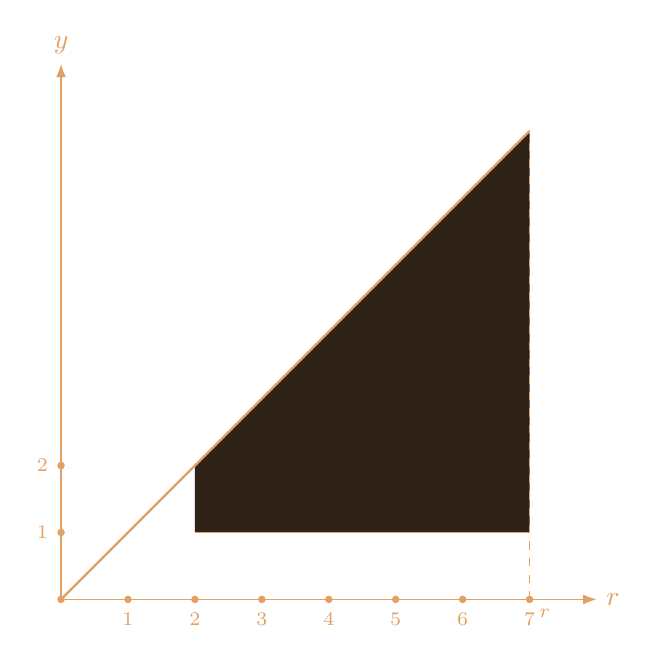
\begin{tikzpicture}[color=orangeText, >=Latex, scale=0.85]

    \def\R{7}

    % shaded region {(x,y): 2<=x<=r, 1<=y<=x}
    \fill[orangeDim!28!black] (2,1) -- (\R,1) -- (\R,\R) -- (2,2) -- cycle;

    % axes
    \draw[->] (0,0) -- (\R+1,0) node[right] {$r$};
    \draw[->] (0,0) -- (0,\R+1) node[above] {$y$};

    % diagonal y = x
    \draw[thick] (0,0) -- (\R,\R);

    % boundary of the shaded region
    \draw (2,1) -- (\R,1);
    \draw[dashed] (\R,0) -- (\R,\R);

    % lattice points
    \foreach \i in {0,1,...,7} {
        \fill (\i,0) circle (1.6pt);
    }
    \fill (0,1) circle (1.6pt);
    \fill (0,2) circle (1.6pt);

    % tick labels
    \foreach \i in {1,2,...,7} {
        \node[below] at (\i,-0.05) {\scriptsize \i};
    }
    \node[left] at (-0.05,1) {\scriptsize $1$};
    \node[left] at (-0.05,2) {\scriptsize $2$};
    \node[below right] at (\R,0) {\scriptsize $r$};

\end{tikzpicture}
\end{document}
